\documentclass[11pt, a4paper]{article}
\usepackage{fullpage}
\usepackage[USenglish]{babel}
\usepackage{graphicx} 
\usepackage[small,bf,hang]{caption2}
\usepackage{hyperref}
\hypersetup{
    colorlinks,
    citecolor=black,
    filecolor=black,
    linkcolor=black,
    urlcolor=black
}

\title{Master Thesis -  Security Aspects in Virtual Networks\\ \textbf{SITREP 12}}
\author{\textbf{Laurent De Wilde} \\ Master of Science in the Applied Computer Science \\ Vrije Universiteit Brussel}
\date{March 30, 2015}

\begin{document}
\maketitle

\section*{Work done}

This is an overview of the work performed in the past week:
\begin{itemize}
\item Performed additional Snort testing on the virtual networks.
\item Completed the final thesis document with the work performed last week. 
\item Made an appointment with Fei Guan concerning the tower server.
\item Transported this machine to my home by car.
\item Performed a dual-boot installation on the tower server I received from the EMS Lab.
\end{itemize}

\section*{Additional Snort testing on the virtual networks}

Last week, I confirmed the correct working of Snort and performed some basic testing with it. Now, advanced testing took place, based on my previous experiece with penetration testing in the OSSEC course. \\
Note that in addition to the standard rules available in Snort, I added approximately 10,000 additional rules to the rules database.

\subsection*{NMAP scanning}

First, some NMAP scanning was performed for reconnaisance of open ports and running services of the target hosts. I started with an unfragmented scan on a Hyper-V VM from the webserver. \\ \\
\noindent\begin{minipage}{\textwidth}
    \centering
    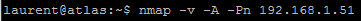
\includegraphics{Ping_Unfragmented_putty.png}
    \captionof{figure}{The NMAP command as executed on the webserver (atlas, 192.168.1.11).}
\end{minipage}
\noindent\begin{minipage}{\textwidth}
    \centering
    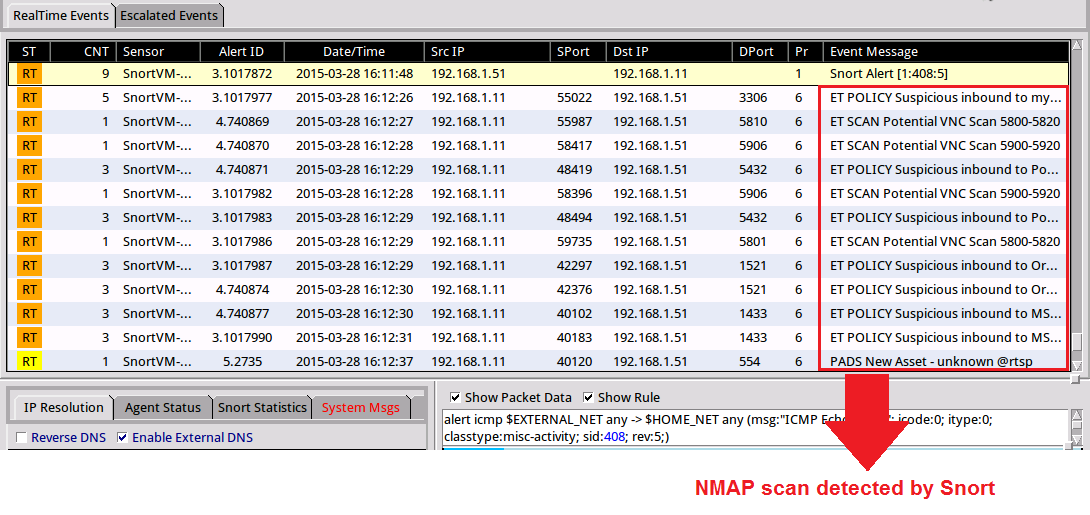
\includegraphics[width=\textwidth]{Ping_Unfragmented.png}
    \captionof{figure}{Basic, unfragmented NMAP scanning of a Hyper-V VM (192.168.1.51). The SnortVM has the IP address of 192.168.1.50. Snort reports each attempt to scan a particular port number.}
\end{minipage}
Next, I performed an NMAP scan with fragmented packets, which splits up the TCP header over several tiny packets to trick / fool IDSs and firewalls. \\ \\
The NMAP command executed is the following: \\ \\
\noindent\begin{minipage}{\textwidth}
    \centering
    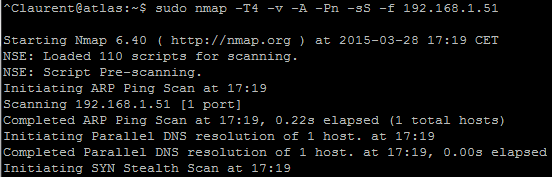
\includegraphics{Ping_Fragmented_2_putty.png}
    \captionof{figure}{The NMAP stealth, SYN packet command as executed on the webserver (atlas, 192.168.1.11).}
\end{minipage}
$\;$ \\ \\
Just as in the OSSEC mini project, the stealth, fragmented scan ICMP ping scan is not detected by Snort. However, Snort did detect the scan for running services as can be seen in the following screen capture. \\ \\
\noindent\begin{minipage}{\textwidth}
    \centering
    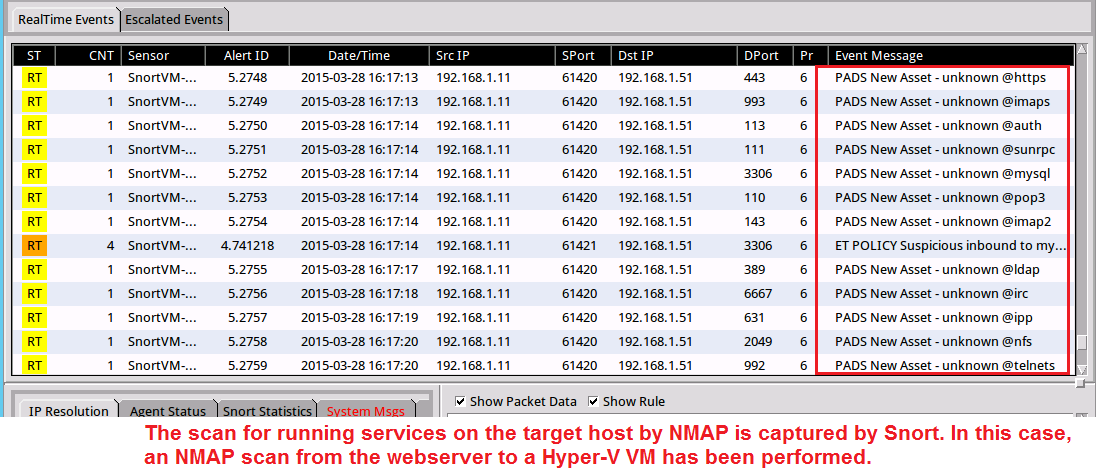
\includegraphics[width=\textwidth]{Ping_Fragmented.png}
    \captionof{figure}{The scan for running services from the stealth scan is detected by Snort.}
\end{minipage}
$\;$ \\ \\
\noindent\begin{minipage}{\textwidth}
    \centering
    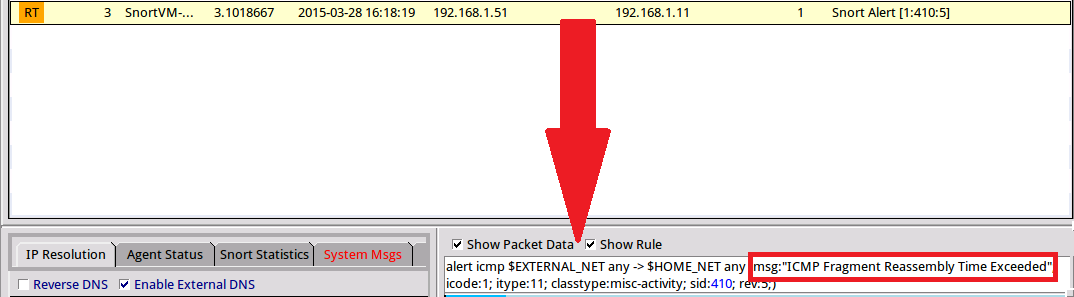
\includegraphics[width=\textwidth]{Ping_Fragmented_2.png}
    \captionof{figure}{However, this Snort alert indicates that a host reassembling a fragment datagram cannot complete the reassembly due to missing fragments whitin the time limit (60s by default). However, I'm not sure whether this is Snort warning for a fragmented / stealth scan.}
\end{minipage}
$\;$ \\ \\
Then I performed an ICMP ping to the Hyper-V VM (192.168.1.51) with a size of 1000 bytes. This gets detected by Snort right away. \\ \\
\noindent\begin{minipage}{\textwidth}
    \centering
    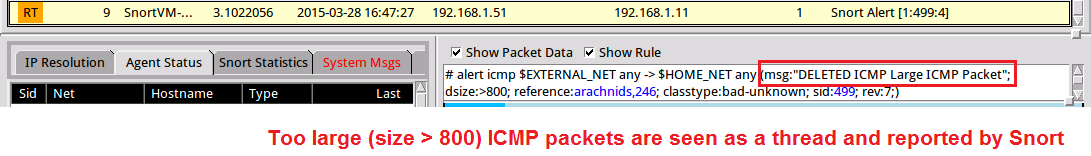
\includegraphics[width=\textwidth]{Ping_Large.png}
    \captionof{figure}{ICMP ping with large packet size is detected by Snort.}
\end{minipage}
$\;$ \\ \\
\noindent\begin{minipage}{\textwidth}
    \centering
    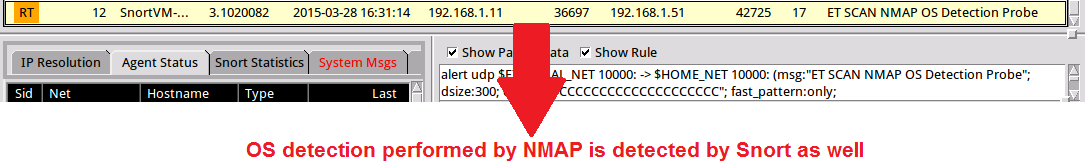
\includegraphics[width=\textwidth]{OS_Detection.png}
    \captionof{figure}{OS detection from a NMAP scan is also detected by Snort.}
\end{minipage}

\subsection*{FTP server attacks}

Next, some attacks on the FTP server running on a Xen virtual network are executed to see how Snort reacts on this. The FPT server has IP address 192.168.1.16 and runs on a Xen VM called ``farbauti''. The client computer has the IP address 192.168.1.40. \\
Remember that the Snort VM runs on the Hyper-V network and has IP address of 192.168.1.50. \\ \\
\noindent\begin{minipage}{\textwidth}
    \centering
    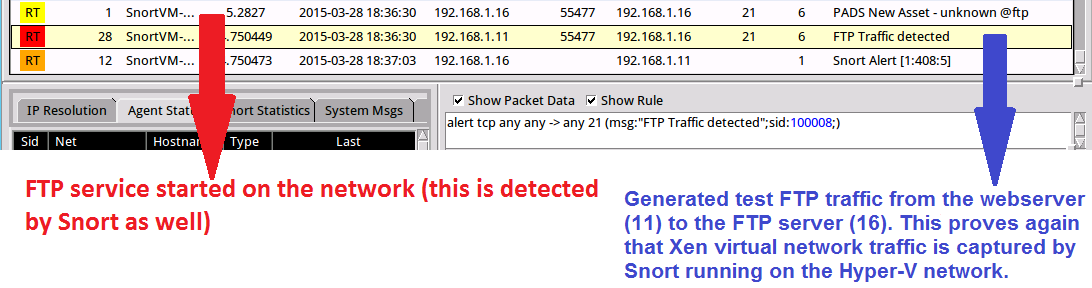
\includegraphics[width=\textwidth]{FTP_1.png}
    \captionof{figure}{First, I created a rule to actually detect FTP traffic as I plan to DOS attack the FTP server is a later stage. The starting of the FTP service and some FTP traffic are detected by Snort.}
\end{minipage}
$\;$ \\ \\
\noindent\begin{minipage}{\textwidth}
    \centering
    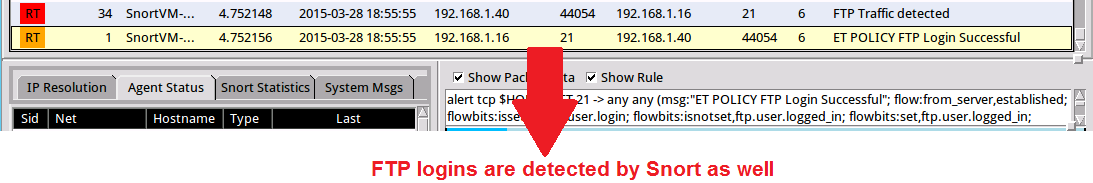
\includegraphics[width=\textwidth]{FTP_2.png}
    \captionof{figure}{Successful FTP logins are also detected by Snort (however, this is not a thread and can be disabled by simply comment the rule that triggered the alert.}
\end{minipage}
$\;$ \\ \\
\noindent\begin{minipage}{\textwidth}
    \centering
    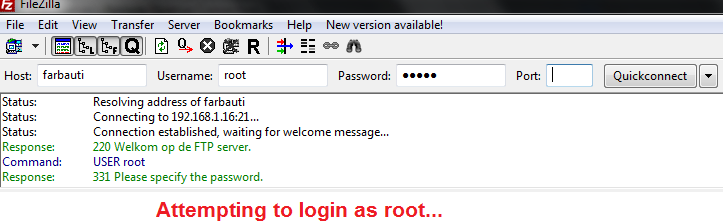
\includegraphics[width=\textwidth]{FTP_4.png}
    \captionof{figure}{Attempting to login as root.}
\end{minipage}
$\;$ \\ \\
\noindent\begin{minipage}{\textwidth}
    \centering
    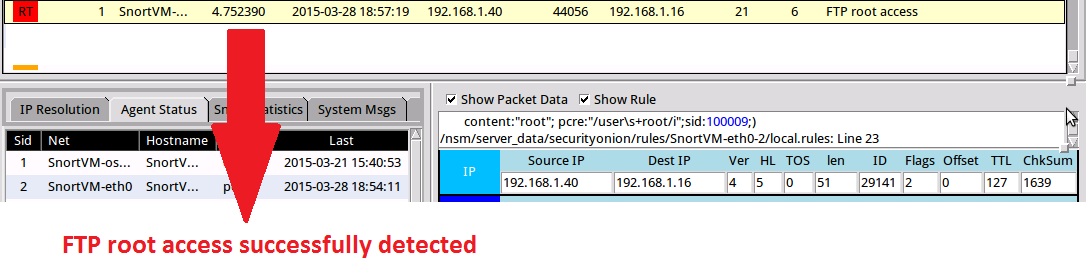
\includegraphics[width=\textwidth]{FTP_3.png}
 \captionof{figure}{FTP root access is successfully detected.}
\end{minipage}
$\;$ \\ \\
For the actual FTP server attacks, I used Metasploit's db\_autopwn command on port 21 on target host 192.168.1.16. \\ \\
\noindent\begin{minipage}{\textwidth}
    \centering
    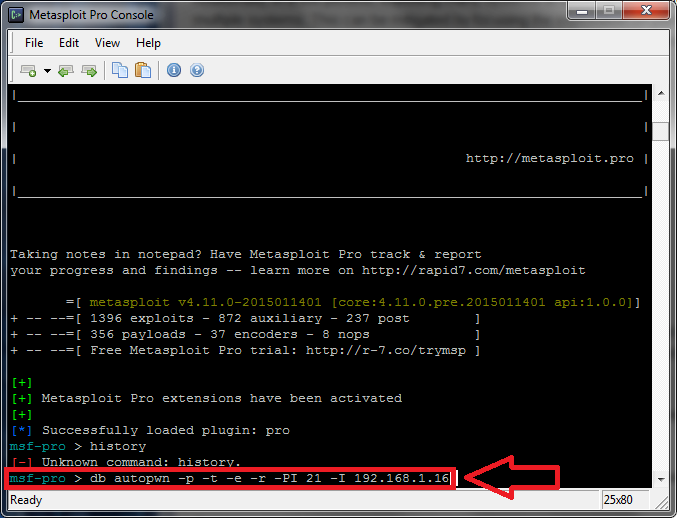
\includegraphics[width=\textwidth]{FTP_6.png}
 \captionof{figure}{The command to attack the FTP server as seen in Metasploit.}
\end{minipage}
$\;$ \\ \\
\noindent\begin{minipage}{\textwidth}
    \centering
    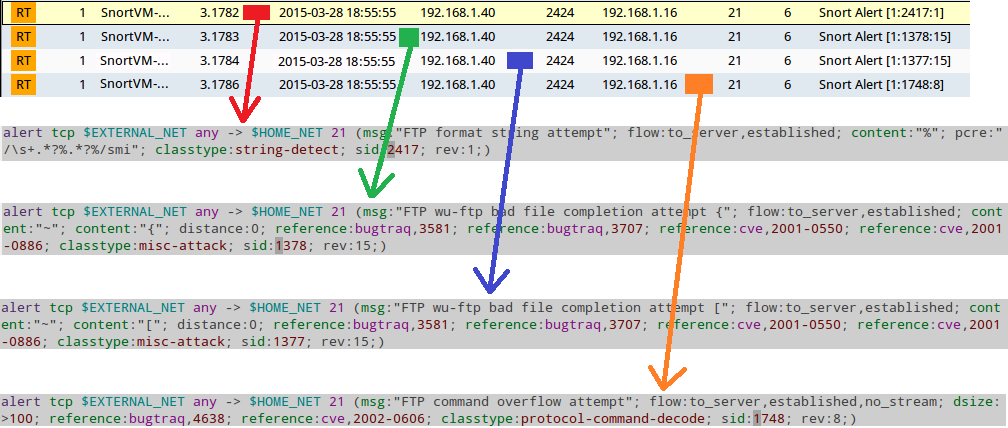
\includegraphics[width=\textwidth]{FTP_5.png}
 \captionof{figure}{Snort reported the various attacks.}
\end{minipage}

\subsection*{SSH attacks}

There was no need to simulate an SSH attack, as the next screen capture reveals: \\ \\
\noindent\begin{minipage}{\textwidth}
    \centering
    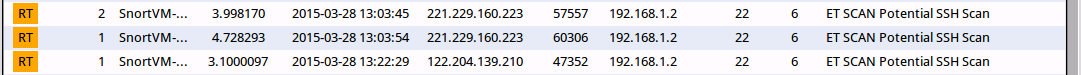
\includegraphics[width=\textwidth]{SSH.png}
 \captionof{figure}{Appearantly, someone tried to SSH scan my Xen server\ldots. This was fortunately detected by Snort.}
\end{minipage}

\subsection*{Database server attacks}

I executed a scan for MySQL databases on the network, as well as commands to show the available databases on the server and root login.

For the database scan, I again used Metasploit. The IP address of the MySQL server is 192.168.1.23 and the MySQL service runs on a Xen VM. \\ \\
\noindent\begin{minipage}{\textwidth}
    \centering
    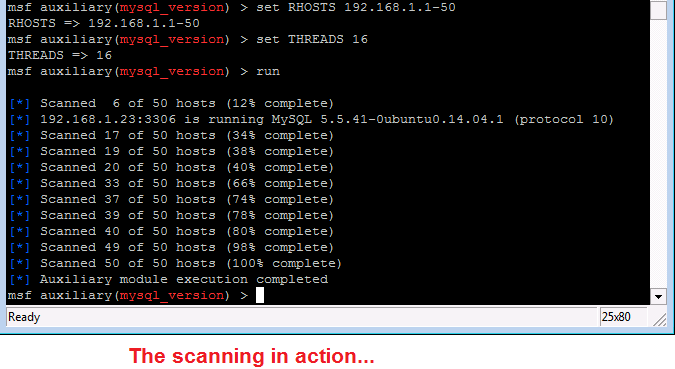
\includegraphics[width=\textwidth]{MySQL_3.png}
 \captionof{figure}{Metasploit is scanning the network for databases...}
\end{minipage}
$\;$ \\ \\
\noindent\begin{minipage}{\textwidth}
    \centering
    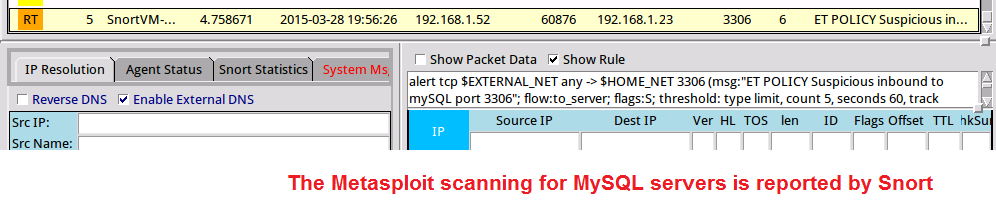
\includegraphics[width=\textwidth]{MySQL_1.png}
 \captionof{figure}{... and this is detected by Snort.}
\end{minipage}
$\;$ \\ \\
Then I executed the ``show databases'' on the terminal of one of the Xen VM's. \\ \\
\noindent\begin{minipage}{\textwidth}
    \centering
    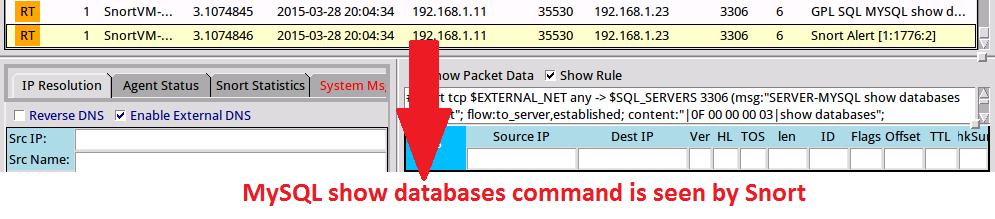
\includegraphics[width=\textwidth]{MySQL_2.png}
 \captionof{figure}{This is captured by Snort.}
\end{minipage}
\noindent\begin{minipage}{\textwidth}
    \centering
    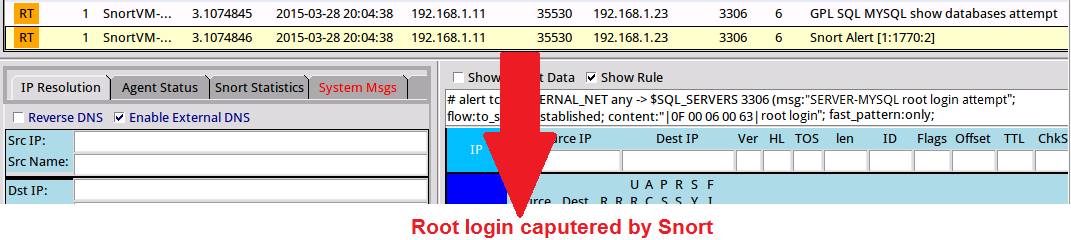
\includegraphics[width=\textwidth]{MySQL_4.png}
 \captionof{figure}{Also logging in a root is detected by Snort.}
\end{minipage}

\subsection*{Trojan Infections}

I created a Trojan Horse to test Snort against Trojan infections and to prove that the default settings of Windows Firewall are not secure enough. The Trojan is a program with a malicious payload that is created on my computer (the attacker), is transfered to the victim and executed by an ordinary user who thinks the program is harmless. \\ \\
I misuse the fact that the default setting of Windows Firewall allows all outbound connections: I make use of reverse TCP, which means that the victim establishes the connetion to the attacker, instead of the other way around (because incoming access is blocked by Windows Firewall). \\ \\
\noindent\begin{minipage}{\textwidth}
    \centering
    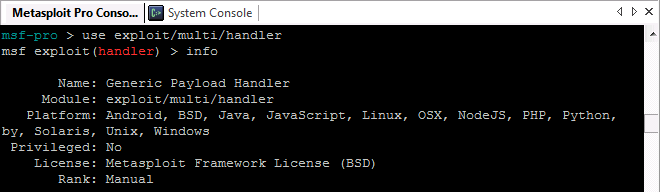
\includegraphics[width=\textwidth]{Trojan_1.png}
 \captionof{figure}{The plugin to create the malicious payload.}
\end{minipage}
$\;$ \\ \\
\noindent\begin{minipage}{\textwidth}
    \centering
    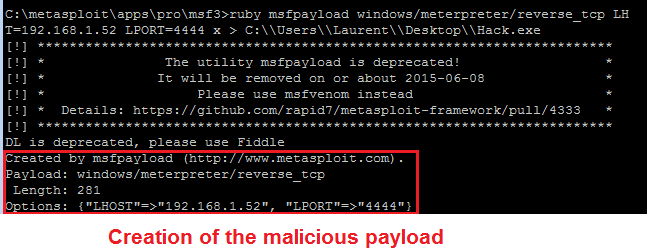
\includegraphics[width=\textwidth]{Trojan_2.png}
 \captionof{figure}{The actual creation of the malicious payload. The ``LHOST'' stands for Local HOST and indicates that the trojan makes a connection with my (attacking) computer via port 4444.}
\end{minipage}
$\;$ \\ \\
\noindent\begin{minipage}{\textwidth}
    \centering
    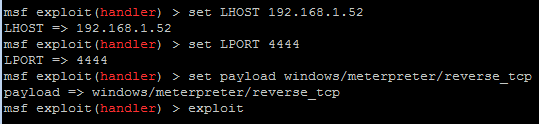
\includegraphics[width=\textwidth]{Trojan_3.png}
 \captionof{figure}{Preparing the listener for when an unsuspicious user clicks on the file.}
\end{minipage}
$\;$ \\ \\
\noindent\begin{minipage}{\textwidth}
    \centering
    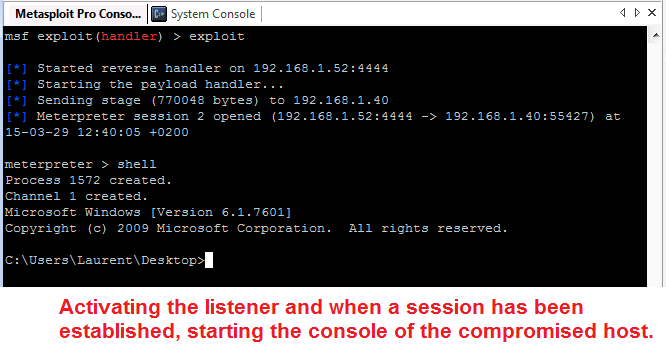
\includegraphics[width=\textwidth]{Trojan_4.png}
 \captionof{figure}{A user clicks on the file and a connection between my computer and the victim is established.}
\end{minipage}
$\;$ \\ \\
\noindent\begin{minipage}{\textwidth}
    \centering
    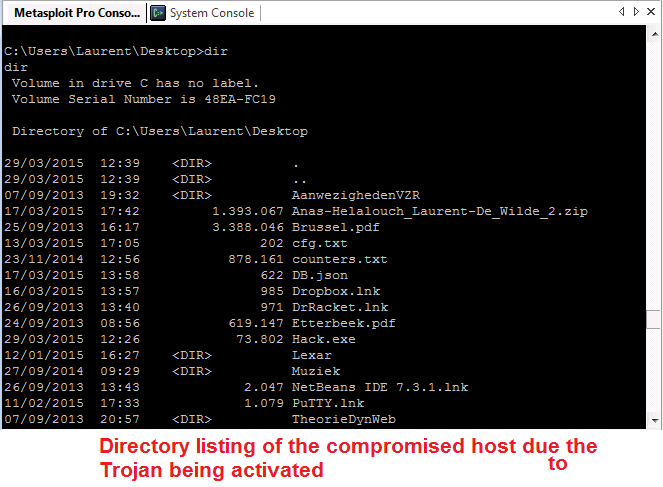
\includegraphics[width=\textwidth]{Trojan_5.png}
 \captionof{figure}{Now I can for example browse the hard disk drive of the victim's computer\ldots}
\end{minipage}
$\;$ \\ \\
\noindent\begin{minipage}{\textwidth}
    \centering
    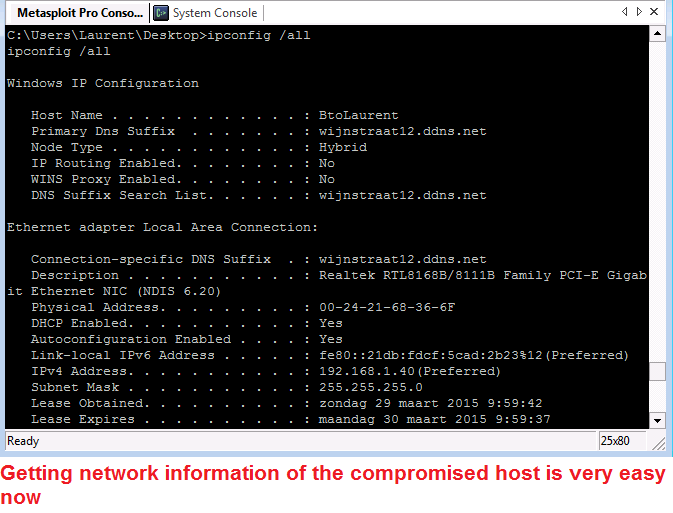
\includegraphics[width=\textwidth]{Trojan_7.png}
 \captionof{figure}{\ldots or obtain some network information to prepare for subsequent attacks.}
\end{minipage}
$\;$ \\ \\
\noindent\begin{minipage}{\textwidth}
    \centering
    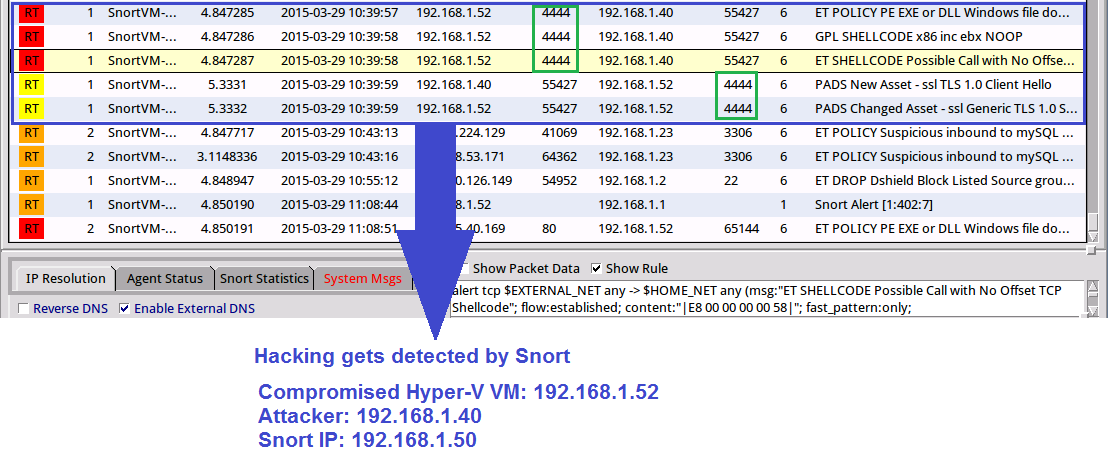
\includegraphics[width=\textwidth]{Trojan_6.png}
 \captionof{figure}{Fortunately, this is detected by Snort.}
\end{minipage}
$\;$ \\ \\
Creating this Trojan, I proved that it possible the get around the Windows Firewall and that also the outbound connections must be restricted.

\subsection*{DOS attacks}

Using LOIC (Low Orbit Cannon), I performed a DOS attack on an FTP - and HTTP server. \\ \\
\noindent\begin{minipage}{\textwidth}
    \centering
    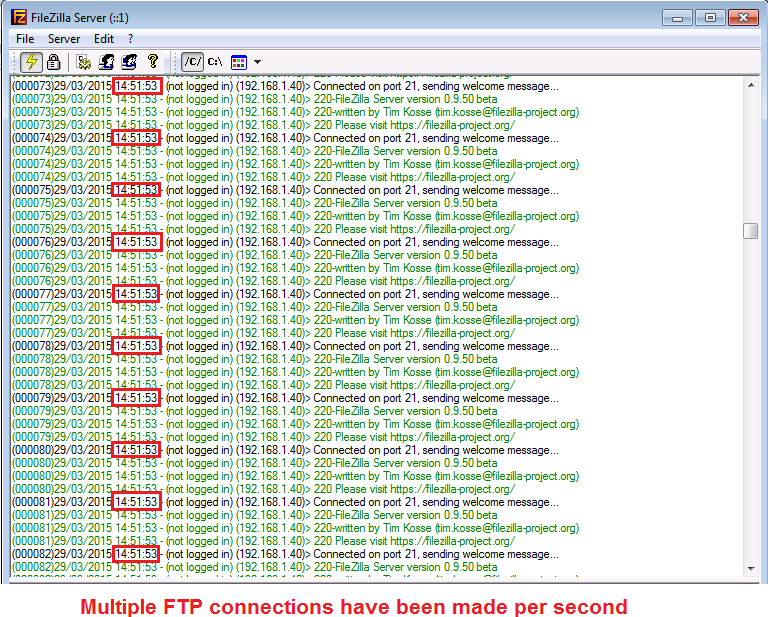
\includegraphics[width=\textwidth]{DOS_2.png}
 \captionof{figure}{The FTP server receives a lot of login attemps per second. This way, we hope to flood it and eventually make it go offline.}
\end{minipage}
$\;$ \\ \\
\noindent\begin{minipage}{\textwidth}
    \centering
    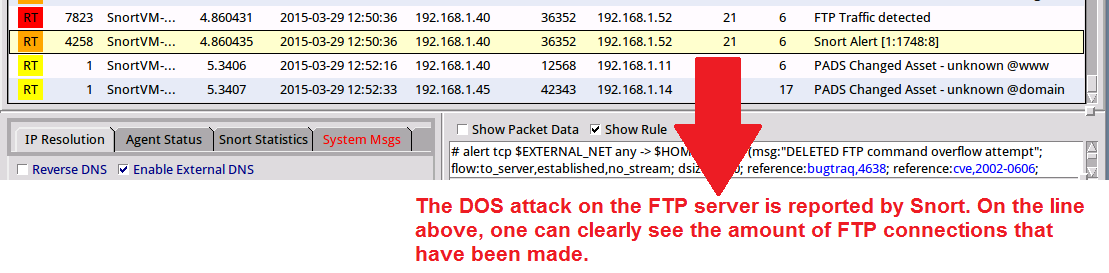
\includegraphics[width=\textwidth]{DOS.png}
 \captionof{figure}{Snort reacts.}
\end{minipage}
$\;$ \\ \\
\noindent\begin{minipage}{\textwidth}
    \centering
    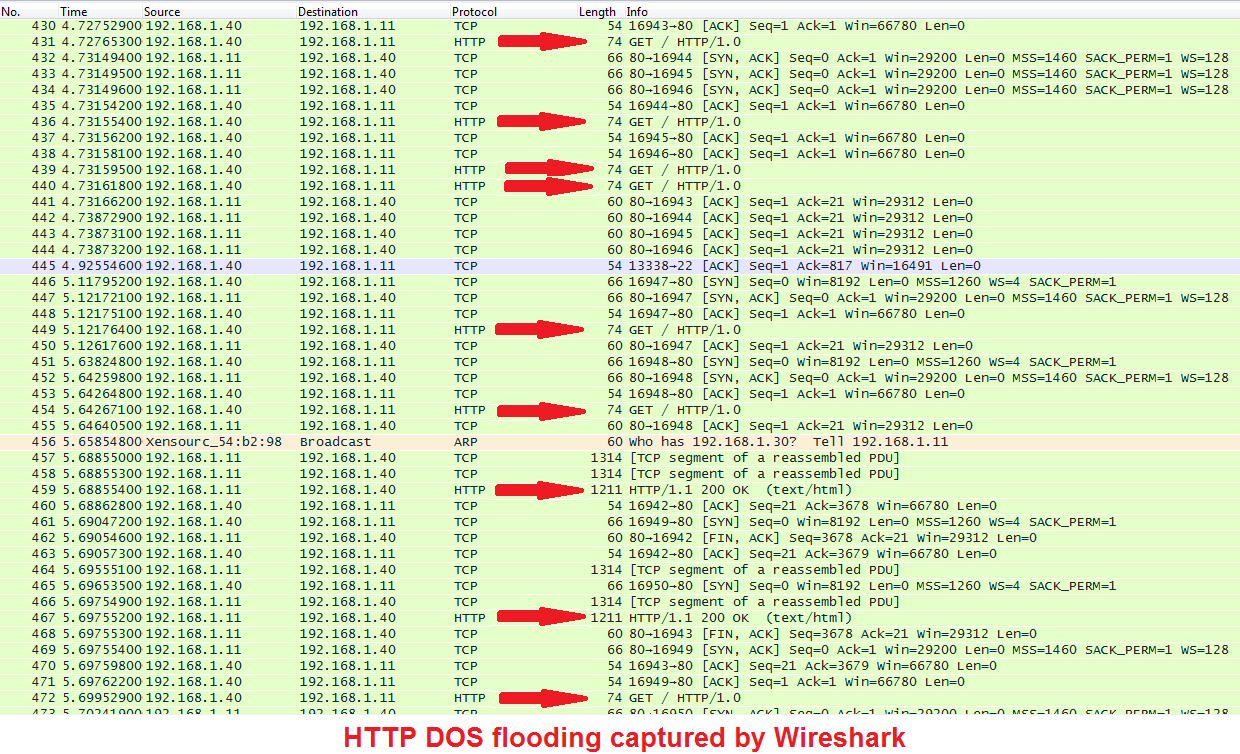
\includegraphics[width=\textwidth]{DOS_4.png}
 \captionof{figure}{The DOS attack on the webserver in action\ldots}
\end{minipage}
$\;$ \\ \\
\noindent\begin{minipage}{\textwidth}
    \centering
    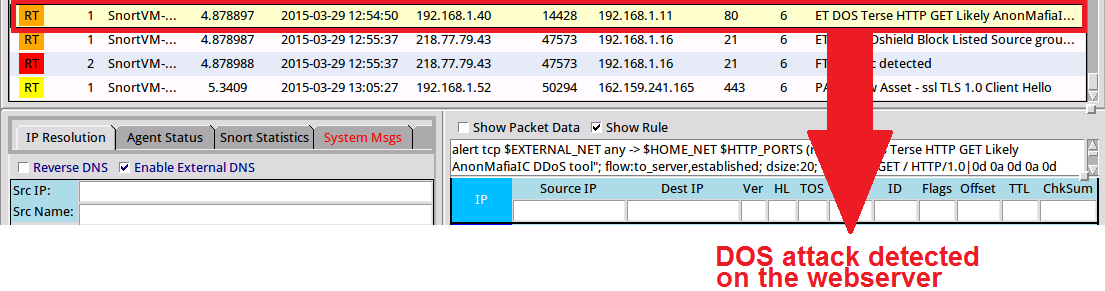
\includegraphics[width=\textwidth]{DOS_3.png}
 \captionof{figure}{Fortunately, this is detected by Snort.}
\end{minipage}

\clearpage

\subsection*{Random stuff}

In this section, some Snort activity that occured regardless of the testing purposes is reported. \\ \\

\noindent\begin{minipage}{\textwidth}
    \centering
    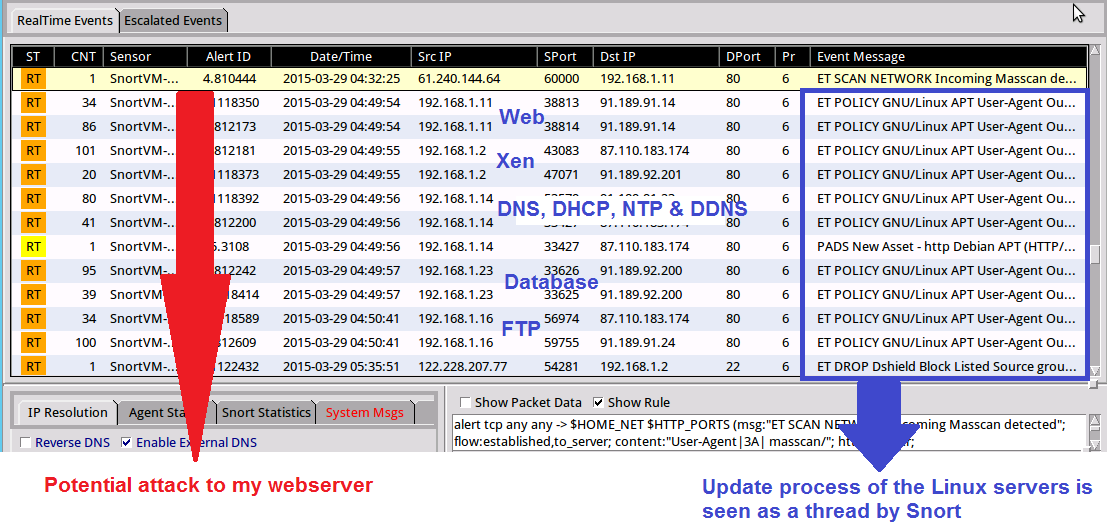
\includegraphics[width=\textwidth]{Random_1.png}
 \captionof{figure}{The apt updating process is seen as a thread by Snort.}
\end{minipage}
$\;$ \\ \\
\noindent\begin{minipage}{\textwidth}
    \centering
    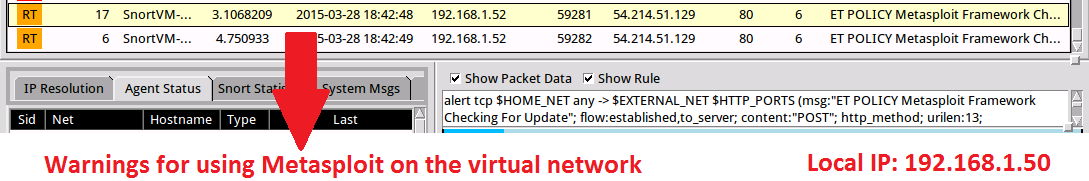
\includegraphics[width=\textwidth]{Metasploit_1.png}
 \captionof{figure}{Metasploit's updating process is known by Snort\ldots}
\end{minipage}
$\;$ \\ \\
\noindent\begin{minipage}{\textwidth}
    \centering
    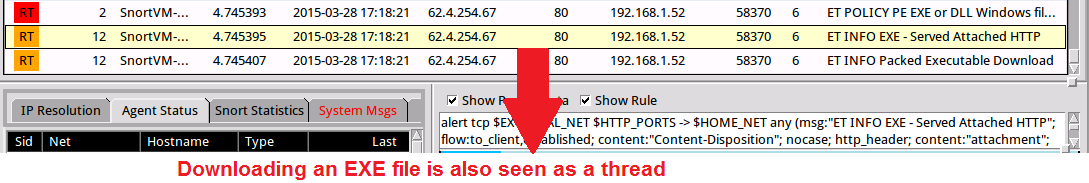
\includegraphics[width=\textwidth]{Exe.png}
 \captionof{figure}{Downloading an .exe file from the Internet is also seen and reported by Snort.}
\end{minipage}
$\;$ \\ \\
Having performed those tests, I have proven that Snort works perfectly on a mixed environment with physical Windows machines, Linux machines, a Xen virtual network and a Hyper-V virtual network.

Of course, the proper configuration must be made prior to using Snort is such an environment, as I have performed in the previous weeks.

\section*{Planning}

This week, I would like to begin hacking a virtual hard disk and see if I can place a virus in it.

\section*{Problems}

No worth mentioning problems were encountered.

\section*{Issues}

On the 1U pizzaserver, I recently noticed that one of harddisk LED's is not blinking anymore. So instead of three LED's blinking, only two are blinking now. However, the disk still makes a spinning noise.

Upon the installation, all three the disks appeared normal in the RAID configuration tool. Perhaps one disk broke down on the two months timespan\ldots .\\
If the Prof would like so, I can further investigate the problem (I have not done this so far).


\section*{Assistance}

No assistance required so far.

However, I did not perform all the attacks / penetration testing on the virtual networks as I did for the OSSEC course. If the Prof desires, I can of course always do some additional testing, but I have proven that Snort indeed works on a Hyper-V virtual network in combination with a Xen virtual network.


\end{document}